\documentclass{llncs}
%%%%%%%%%%%%%%%%%%%%%%%%%%%%%%%%%%%%%%%%%%%%%%%%%%%%%%%%%%%
%% package sillabazione italiana e uso lettere accentate
\usepackage[latin1]{inputenc}
\usepackage[english]{babel}
\usepackage[T1]{fontenc}
%%%%%%%%%%%%%%%%%%%%%%%%%%%%%%%%%%%%%%%%%%%%%%%%%%%%%%%%%%%%%

\usepackage{url}
\usepackage{xspace}
\usepackage{listings}
\usepackage{hyperref}
\usepackage{caption}
\usepackage{subfigure}


\makeatletter
%%%%%%%%%%%%%%%%%%%%%%%%%%%%%% User specified LaTeX commands.
\usepackage{manifest}

\makeatother

%%%%%%%
 \newif\ifispdf
 \ifx\pdfoutput\undefined
 \ispdffalse % we are not running PDFLaTeX
 \else
 \pdfoutput=1 % we are running PDFLaTeX
 \ispdftrue
 \fi
%%%%%%%
 \ifispdf
 \usepackage[pdftex]{graphicx}
 \else
 \usepackage{graphicx}
 \fi
%%%%%%%%%%%%%%%
 \ifispdf
 \DeclareGraphicsExtensions{.pdf, .jpg, .tif, .eps}
 \else
 \DeclareGraphicsExtensions{.eps, .jpg}
 \fi
%%%%%%%%%%%%%%%

\newcommand{\action}[1]{\texttt{#1}\xspace}
\newcommand{\code}[1]{{\small{\texttt{#1}}}\xspace}
\newcommand{\codescript}[1]{{\scriptsize{\texttt{#1}}}\xspace}

% Cross-referencing
\newcommand{\labelsec}[1]{\label{sec:#1}}
\newcommand{\xs}[1]{\sectionname~\ref{sec:#1}}
\newcommand{\xsp}[1]{\sectionname~\ref{sec:#1} \onpagename~\pageref{sec:#1}}
\newcommand{\labelssec}[1]{\label{ssec:#1}}
\newcommand{\xss}[1]{\subsectionname~\ref{ssec:#1}}
\newcommand{\xssp}[1]{\subsectionname~\ref{ssec:#1} \onpagename~\pageref{ssec:#1}}
\newcommand{\labelsssec}[1]{\label{sssec:#1}}
\newcommand{\xsss}[1]{\subsectionname~\ref{sssec:#1}}
\newcommand{\xsssp}[1]{\subsectionname~\ref{sssec:#1} \onpagename~\pageref{sssec:#1}}
\newcommand{\labelfig}[1]{\label{fig:#1}}
\newcommand{\xf}[1]{\figurename~\ref{fig:#1}}
\newcommand{\xfp}[1]{\figurename~\ref{fig:#1} \onpagename~\pageref{fig:#1}}
\newcommand{\labeltab}[1]{\label{tab:#1}}
\newcommand{\xt}[1]{\tablename~\ref{tab:#1}}
\newcommand{\xtp}[1]{\tablename~\ref{tab:#1} \onpagename~\pageref{tab:#1}}

% Category Names
\newcommand{\sectionname}{Section}
\newcommand{\subsectionname}{Subsection}
\newcommand{\sectionsname}{Sections}
\newcommand{\subsectionsname}{Subsections}
\newcommand{\secname}{\sectionname}
\newcommand{\ssecname}{\subsectionname}
\newcommand{\secsname}{\sectionsname}
\newcommand{\ssecsname}{\subsectionsname}
\newcommand{\onpagename}{on page}

\newcommand{\xauthA}{Luca Mella}
\newcommand{\xauthB}{NameB StudentB}
\newcommand{\xauthC}{NameC StudentC}
\newcommand{\xfaculty}{II Faculty of Engineering}
\newcommand{\xunibo}{Alma Mater Studiorum -- University of Bologna}
\newcommand{\xaddrBO}{viale Risorgimento 2}
\newcommand{\xaddrCE}{via Venezia 52}
\newcommand{\xcityBO}{40136 Bologna, Italy}
\newcommand{\xcityCE}{47521 Cesena, Italy}




\begin{document}

\title{Simulation Report\\Progetto Reti 2013}

\author{\xauthA}

\institute{
\xunibo\\\xaddrCE, \xcityCE\\\email\ luca.mella@studio.unibo.it
}

\maketitle

%\tableofcontents



%===========================================================================
\section{M/D/1 and M/M/1 comparison}
\labelsec{MD1_MM1}
In order to support MD1 system's simulations we slightly modify provided simulator source code for supporting multiple service time distribution.\\
We created a service time distribution agnostic simulation core which can be easily extended with arbitrary distribution. The complete source code can be found at \url{https://github.com/luca-m/ProgRetiLM1213/blob/master/sim/xx1prio.c}

\lstset{language=C, caption=MD1 simulator extension,  basicstyle=\ttfamily\scriptsize , breaklines=true}
\lstinputlisting{../sim/md1prio.c}

\subsection{Simulations details}
In general simulation data have been obtained though multiple run of the same experiment using different seed for feeding the PRNG\footnote{We also used different PRNG form original simulation implementation. We integrated an implementation of the \emph{Mersenne-Twist} PRNG, which is known for its better quality.}.\\
In order to obtain relevant statistical data we performed 50 run of the same experiment, where experiment is meant to have unique input parameters (eg. same rho).\\
Experimental data have been processed further in order to extract the 95\% confidence interval boundaries. Further details about implementation are freely available at \url{https://github.com/luca-m/ProgRetiLM1213/blob/master/sim/sim1.sh} and \url{https://github.com/luca-m/ProgRetiLM1213/blob/master/sim/sim2.sh}

%===========================================================================
\subsection{Fixed $\rho$ and $\mu$}
\labelsec{MD1_MM1_fixed_rho}

As suggested in specification, we first run a simulation's battery with fixed $\rho$ and $\mu$, varying the number of arrivals in the system and showing $\eta$ mean with its related confidence interval.

\begin{figure}
\centering
\includegraphics[width=0.8\textwidth]{../sim/results/1/md1_fixed_rho.pdf}
\caption{MD1 with fixed $\rho$ and $\mu$.}
\label{fig:md1_fixed}
\end{figure}

In fig.\ref{fig:md1_fixed} is possible to note that MD1 is quite insensitive to the number of arrivals, at least if simulation lasts sufficiently (minimum 100 arrivals).\\
In fig.\ref{fig:mm1_fixed}, where MM1 simulation's result s are shown, we note that this kind of service distribution is not insensitive like the previous one. A possible explanation of this behaviour could reside in the presence of variability that characterize MM1, and dually in the complete lack of variability which is a typical feature of MD1.
 
\begin{figure}
\centering
\includegraphics[width=0.8\textwidth]{../sim/results/1/mm1_fixed_rho.pdf}
\caption{MM1 with fixed $\rho$ and $\mu$.}
\label{fig:mm1_fixed}
\end{figure}


%===========================================================================
\subsection{Variable $\rho$}
\labelsec{MD1_MM1_fixed_rho}

In this set of experiments we had variate $\rho$ across the interval $[0,1)$, $500$ arrivals, and mean service time $\vartheta=3$.\\
Then we performed a comparison between simulation outcomes and analytical results.\\

\begin{figure}
\begin{minipage}[b]{7cm}
\centering
\includegraphics[width=7cm]{../sim/results/1/md1_var_rho.pdf}
\end{minipage}\qquad
\begin{minipage}[b]{7cm}
\centering
\includegraphics[width=7cm]{../sim/results/1/mm1_var_rho.pdf}
\end{minipage}
\caption{MD1 and MM1 with confidence interval 95\%}
\label{fig:md1_mm1_varrho_confint}
\end{figure}

The figures \ref{fig:md1_mm1_varrho_confint} show simulated $\eta$ mean with different $\rho$ values, with emphasis on confidence interval, which remain pretty close to the average value. This mean that the simulation parameters chosen are good enough for our purposes.\\
In fig.\ref{fig:md1_mm1_varrho_compare} we focus on the ratio between MM1 and MD1 $\eta$ mean. It can be noted that simulated results show the same motif of the theoretical ones, in fact the delay introduced by MD1 is approximately $\frac{1}{2} \cdot avg(\eta_ {MM1})$, just as suggested by analytical results seen during the lectures.

\begin{figure}
\begin{minipage}[b]{7.5cm}
\centering
\includegraphics[width=7.5cm]{../sim/results/1/mm1_md1_sim.pdf}
\end{minipage}\qquad
\begin{minipage}[b]{7.5cm}
\centering
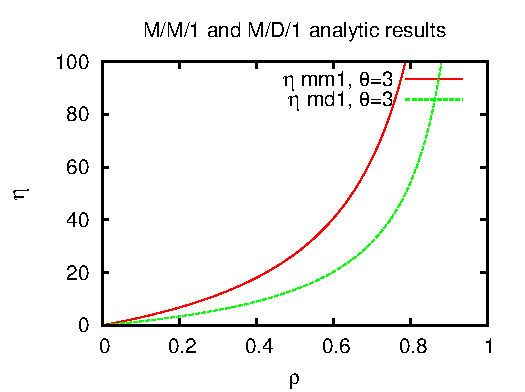
\includegraphics[width=7.5cm]{../sim/results/1/mm1_md1_theorical.pdf}
\end{minipage}
\caption{Simulated results compared with analytical results}
\label{fig:md1_mm1_varrho_compare}
\end{figure}


\newpage
%===========================================================================
\section{M/G/1//PRIO}
\labelsec{MG1PRIO}

In this section we report the outcomes many simulations of distinct M/G/1/Prio systems, each one with $\rho \in [0,1)$, $500$ arrivals, $50$ samples per experiment, and different relationship between $rho_i$ of each priority level.


%===========================================================================
\subsection{Two class of service}
\labelsec{MG1PRIO_2class}

The simulated system is characterized by a M/M/1/Prio system with the following relationship between utilization factors:
\begin{center}
$\rho_1 = x \cdot \rho $\\
$\rho_2 = (1-x) \cdot \rho $\\
$\rho \in [0,1)$\\
\end{center}

In fig.\ref{fig:mm1_2class_all} are reported the average wait times for service class 1 and 2, and also the global wait time of the system, which is equivalent to the wait time we could measure in a M/M/1 system with the same $\rho$.\\
We can note that service class 2 users are highly penalized when $\rho$ is moving getting greater than $0.5$.\\
If the reader is interested in further detail about confidence intervals we invite him to visit \url{https://github.com/luca-m/ProgRetiLM1213/tree/master/sim/results} where a more exhaustive collection of plots can be found.

\begin{figure}
\centering
\includegraphics[width=0.65\textwidth]{../sim/results/2/mm1_2class_all.pdf}
\caption{Average wait time in M/M/1/Prio with 2 class of services, $\rho \in [0,1)$.}
\label{fig:mm1_2class_all}
\end{figure}
\newpage
%===========================================================================
\subsection{Three class of service, case 1}
\labelsec{MG1PRIO_3class_1}

The simulated system is characterized by a M/M/1/Prio system with the following relationship between utilization factors:

\begin{center}
$\rho_1 = \frac{x}{2} \cdot \rho $\\
$\rho_2 = \rho_1$ \\
$\rho_3 = (1-x) \cdot \rho$\\
$\rho \in [0,1)$\\
\end{center}

In fig.\ref{fig:mm1_3class_1_all} can be noted how class 1 and class 2 are advantaged w.r.t. class 3, in fact they have similar wait time until $\rho < 0.5$, when utilization factor grows over $0.8$ class 2 is slightly penalized, meanwhile class 3 users are experimenting high delay and poor quality of service.

\begin{figure}
\centering
\includegraphics[width=0.8\textwidth]{../sim/results/2/mm1_3class_1_all.pdf}
\caption{Average wait time in M/M/1/Prio with 3 class of services, $\rho \in [0,1)$.}
\label{fig:mm1_3class_1_all}
\end{figure}
\newpage
%===========================================================================
\subsection{Three class of service, case 2}
\labelsec{MG1PRIO_3class_2}

The simulated system is characterized by a M/M/1/Prio system with the following relationship between utilization factors:

\begin{center}
$\rho_1 = \frac{x}{10} \cdot \rho $\\
$\rho_2 = 9 \cdot \frac{x}{10} \cdot \rho$\\
$\rho_3 = (1-x) \cdot \rho$\\
$\rho \in [0,1)$ \\
In fig.\ref{fig:mm1_3class_2_all} we note a scenario similar to the previous one. In fact both service class 1 and 2 have lower wait time too, but when $\rho$ is near 1 (which is the theoretical limit for system ergodicity) these 2 class continue to be preserved and maintains average wait time lower than the equivalent M/M/1 system without priority. Obviously service class 3 pay this fact by having higher delay peak.
\end{center}

\begin{figure}
\centering
\includegraphics[width=0.8\textwidth]{../sim/results/2/mm1_3class_2_all.pdf}
\caption{Average wait time in M/M/1/Prio with 3 class of services, $\rho \in [0,1)$.}
\label{fig:mm1_3class_2_all}
\end{figure}
\newpage
%===========================================================================
\subsection{Three class of service, case 3}
\labelsec{MG1PRIO_3class_3}

The simulated system is characterized by a M/M/1/Prio system with the following relationship between utilization factors:
\begin{center}
$\rho_1 = x \cdot \rho $ \\
$\rho_2 = \frac{(1-x)}{2} \cdot \rho$ \\  
$\rho_3 = \rho_2 $ \\
$\rho \in [0,1)  $ \\
\end{center}
As shown in fig.\ref{fig:mm1_3class_3_all} this case is slightly different than the previous ones. Here class 2 users can benefit of their priority just for low utilization factors, in fact when $\rho > 0.5$ the average wait time is higher than in the previous scenarios. With this set-up only class 1 user are experimenting benefits with non trivial workload.

\begin{figure}
\centering
\includegraphics[width=0.8\textwidth]{../sim/results/2/mm1_3class_3_all.pdf}
\caption{Average wait time in M/M/1/Prio with 3 class of services, $\rho \in [0,1)$.}
\label{fig:mm1_3class_3_all}
\end{figure}
\newpage
%===========================================================================
\bibliographystyle{abbrv}
\bibliography{biblio}

\appendix

\section{Data Set and Simulation Scripts}
For sake of completeness additional plots of the described experiments are published at \url{https://github.com/luca-m/ProgRetiLM1213/tree/master/sim/results} where ere are present more detailed plots with 95\% confidence interval.\\
In order to replicate the experiment the reader can found automation scripts \url{https://github.com/luca-m/ProgRetiLM1213/tree/master/sim/sim1.sh} and \url{https://github.com/luca-m/ProgRetiLM1213/tree/master/sim/sim2.sh}.\\
The time distribution agnostic simulator source code at \url{https://github.com/luca-m/ProgRetiLM1213/blob/master/sim/xx1prio.c}. \\
Script used for confidence interval calculation \url{https://github.com/luca-m/ProgRetiLM1213/blob/master/sim/confidence_interval.R} \\
Script used for plotting graph with confidence interval \url{https://github.com/luca-m/ProgRetiLM1213/blob/master/sim/plot_confidence.R}\\
Script used for plots with multiple $\eta$ mean \url{https://github.com/luca-m/ProgRetiLM1213/blob/master/sim/plot_summary.R}


\end{document}












